\chapter{Algorithme de Bellman-Ford}\index{Bellman-Ford (algorithme)}
\vspace*{-0.5cm}
Cet algorithme permet de trouver les plus courts chemins depuis un sommet source donné. Il est cependant moins performant que Dijkstra, mais est distribuable, chaque sommet du réseau connaît ses voisins, propage les résultats des calculs intermédiaires à ses voisins.

\section{Idée}

Commencer avec $d(s)$ = 0 et $d(u) = \infty \ \forall u \neq s$.

À chaque itération, on parcourt toutes les arêtes du graphe; $(u,\, v)\in A$ : si $d(u) + w(u,\, v) < d(v)$

On pose $d(v) = d(u) + w(u,\, v)$ et $pred(v) = u$.

\subsection*{Exemple}

%\SetUpEdge[color=orange,lw=1.5]
\begin{figure}[h]
  \centering
  	\begin{tikzpicture}
		\tikzset{VertexStyle/.append  style={fill = node}}
		\tikzset{VertexStyle/.append  style={text = white}}
		\SetGraphUnit{1.5}
		\Vertex{A}
		\NOEA(A){B}
		\SOEA(A){C}
		\SetGraphUnit{3}
		\EA(B){D}
		\SetGraphUnit{1.5}
		\NOEA(C){E}
		\Edge[label=$2$](A)(B)
		\Edge[label=$12$](A)(C)
		\Edge[label=$8$](B)(C)
		\Edge[label=$4$](B)(D)
		\Edge[label=$1$](B)(E)
		\Edge[label=$1$](C)(E)
		\Edge[label=$2$](D)(E)
		\Edge[style={bend left=60},label=$4$](D)(C)
	\end{tikzpicture}
\end{figure}%


\begin{figure}[h]
\centering
\begin{minipage}{.3\textwidth}
	\centering
  	\begin{tikzpicture}
	$t = 1$
		\tikzset{VertexStyle/.append  style={fill = node}}
		\tikzset{VertexStyle/.append  style={text = white}}
		\SetGraphUnit{1.5}
		\Vertex[x=0, y=1]{A}
		\SetVertexLabelOut
		\tikzset{VertexStyle/.append  style={text = orange}}
		\Vertex[Lpos=90, x=1, y=2]{2}
		\Vertex[Lpos=-90, x=1, y=0]{12}
		\tikzset{VertexStyle/.append  style={text = white}}
		\SetVertexLabelIn
		\Vertex[x=1, y=2]{B}
		\Vertex[x=1, y=0]{C}
		\Edge(A)(B)
		\Edge(A)(C)
	\end{tikzpicture}
\end{minipage}%
\begin{minipage}{.3\textwidth}
	\centering
  	\begin{tikzpicture}
	$t = 2$
		\tikzset{VertexStyle/.append  style={fill = node}}
		\tikzset{VertexStyle/.append  style={text = white}}
		\SetGraphUnit{1.5}
		\Vertex[x=0, y=1]{A}
		\SetVertexLabelOut
		\tikzset{VertexStyle/.append  style={text = orange}}
		\Vertex[Lpos=90, x=1, y=2]{2}
		\Vertex[Lpos=-90, x=1, y=0]{10}
		\Vertex[Lpos=-45, x=2, y=1]{3}
		\Vertex[x=3, y=2]{6}
		\tikzset{VertexStyle/.append  style={text = white}}
		\SetVertexLabelIn
		\Vertex[x=1, y=2]{B}
		\Vertex[x=1, y=0]{C}
		\Vertex[x=2, y=1]{E}
		\Vertex[x=3, y=2]{D}
		\Edge(A)(B)
		\Edge(B)(C)
		\Edge(B)(E)
		\Edge(B)(D)
	\end{tikzpicture}
\end{minipage}%
\begin{minipage}{.3\textwidth}
	\centering
  	\begin{tikzpicture}
	$t = 3$
		\tikzset{VertexStyle/.append  style={fill = node}}
		\tikzset{VertexStyle/.append  style={text = white}}
		\SetGraphUnit{1.5}
		\Vertex[x=0, y=1]{A}
		\SetVertexLabelOut
		\tikzset{VertexStyle/.append  style={text = orange}}
		\Vertex[Lpos=90, x=1, y=2]{2}
		\Vertex[Lpos=-90, x=1, y=0]{4}
		\Vertex[Lpos=-45, x=2, y=1]{3}
		\Vertex[x=3, y=2]{5}
		\tikzset{VertexStyle/.append  style={text = white}}
		\SetVertexLabelIn
		\Vertex[x=1, y=2]{B}
		\Vertex[x=1, y=0]{C}
		\Vertex[x=2, y=1]{E}
		\Vertex[x=3, y=2]{D}
		\Edge(A)(B)
		\Edge(E)(C)
		\Edge(B)(E)
		\Edge(E)(D)
	\end{tikzpicture}
\end{minipage}%
\end{figure}

On remarque qu'à l'itération $t$ on trouve des plus courts chemins qui parcourent au plus $t$ arêtes.

Un plus court chemin de $s$ à $u$ parcourt au plus $n - 1$ arêtes. Pour que l'algorithme soit correct, il suffit de montrer qu'à l'itération $t$ on a calculé les plus courts chemins passant par au plus $t$ arêtes et répéter $n - 1$ fois pour avoir tous les plus courts chemins de $s$ aux autres sommets.

\section{Implémentation en Python}

\lstinputlisting{Scripts/Bellman_Ford.py}

Complexité : $n \times m$


\vspace*{0.2cm}
\section{Preuve}

\begin{definition} On note:

\begin{itemize}
\item $\delta^{t}(u,\, v) = $ longueur du plus court cheminde $u$ à $v$ en passant par au plus $t$ arêtes.
\item $v.dist^{t} = $ valeur de $v.dist$ à l'itération $t$.
\end{itemize}
\end{definition}

\begin{proposition}
$\forall v \in S \ d^{t}(v) = \delta^{t}(s,\, v)$
\end{proposition}

\begin{proof}
Par récurrence sur $t$.

Lorsque $t = 0$, un seul chemin de longueur $0$ de $s$ à $s$.

À l'itération $t > 0$, par hypothèse d'induction, $\forall x \ x.dist^{t-1} = \delta^{t-1}(s,\, x)$

Soit $C_{v}$ un plus court chemin de $s$ à $v$ parcourant au plus $t$ arêtes. Si $C_{v}$ a moins de $t$ arêtes alors on l'a découvert à une itération précédente $t^{\prime} < t$ donc $v.dist^{t^{\prime}} = \delta^{t-1}(s,\, v)$. Si $C_{v}$ a $t$ arêtes, le chemin $s \longrightarrow x$ est un plus court chemin qui parcourt au plus $t - 1$ arêtes (sinon on trouverait un meilleur chemin de $t$ arêtes vers $v$).

On peut appliquer l'hypothèse d'induction $x \ x.dist^{t-1} = \delta^{t-1}(s,\, x)$ .

À l'itération $t$ on considère $x$ et son voisin $v$ et on posera :

\begin{tabular}{l l l}
$v.dist$ & $\leq$ & $x.dist + w(x,\, v)$ \\
	& $=$ & $\delta^{t-1}(s,\, x) + w(x,\, v)$ \\
	& $=$ & $\delta^{t}(s,\, v)$ \\
\end{tabular}
\end{proof}